%% wp3 张量与切片（论文 Tensor/Slicing 小节）
\wpsh{张量（Tensor）}
\label{sec:tensor}

最后，我们定义张量（tensor）——\CuTe 的核心对象——做法是把一个布局（layout）绑定到一个访问器（accessor）上。访问器实际上是面向布局的、支持随机访问的类指针对象。

\begin{definition}
{\em 访问器}（accessor）是支持偏移（offset）与解引用（dereference）操作的对象：
\begin{align*}
e + d &\to e', &&\text{将访问器 $e$ {\bf 偏移}（offset）$d \in \D$，产生另一访问器 $e'$；} \\
*e &\to v, &&\text{{\bf 解引用}（dereference）访问器 $e$，产生值 $v$；} \\
e[d] &\to *(e+d), &&\text{{\bf 下标}（subscript）算符，一种常用的便捷写法。}
\end{align*}
\end{definition}
当 $\D = \Z$ 时，访问器的常见实现包括原始指针（如 \texttt{T*}）、数组（如
\texttt{T[N]}）以及随机访问迭代器（如
\texttt{thrust::\allowbreak{}counting\allowbreak\_iterator} 与
\texttt{thrust::\allowbreak{}transform\allowbreak\_iterator} 等）。当 $\D$ 是更为特殊的整数半模时，访问器必须与该半群的加法运算相容。

\begin{definition}
{\em 张量}（tensor）由访问器 $e$ 与布局 $\v{L}$ 的复合（Composition）所定义，记作 $T = e \circ \v{L}$。张量对布局求值的方式是：把坐标 $c \in \Z(\v{L})$ 映射到陪域 $\D$，据此对访问器做偏移，再对结果解引用，从而得到张量的值。形式化地，
\begin{align}
T(c) = (e \circ \v{L})(c) = *(e + \v{L}(c)) = e[\v{L}(c)],
\label{eqn:tensor}
\end{align}
即得到张量在坐标 $c$ 处的值。
\end{definition}

大多数张量是以内存地址作为访问器的数据布局。例如，内存地址 $p$ 可以作为带普通偏移与解引用操作的指针访问器 $\{p\}$，用来构造数据张量，
\begin{align*}
\{p\} + b &\to \{p+b\} \\
*\{p\} &\to *p \\
T &= \{p\} \circ \v{L}.
\end{align*}
此外，图~\ref{fig:layouts} 中所示的所有布局都可以通过与计数迭代器 $\{a\}$ 复合而变换为隐式张量，该迭代器解引用到所存储的偏移 $a \in \Z$，
\begin{align*}
\{a\} + b &\to \{a+b\} \\
*\{a\} &\to a \\
T &= \{a\} \circ \v{L}.
\end{align*}
类似地，图~\ref{fig:layouts:coord0} 与图~\ref{fig:layouts:coord1} 中所示的坐标布局可以通过与访问器 $\{(a,b)\}$ 复合而变换为隐式张量，该访问器按坐标进行偏移，并解引用到所存储的坐标 $(a,b) \in \Z^{(\star,\star)}$，
\begin{align*}
\{(a,b)\} + (c,d) &\to \{(a+c,b+d)\} \\
*\{(a,b)\} &\to (a,b) \\
T &= \{(a,b)\} \circ \v{L}.
\end{align*}


% \wpssh{$\D$-torsor（$\D$-挠子）}

% 形式上，若集合 $E$ 配备运算 $E + M \to E$（其中 $M$ 是一个群），则称 $E$ 为一个 $M$-torsor。访问器是 $\D$-torsor，可以解引用到另一个集合 $V$，即其值集。例如，指针是一个 $\Z$-torsor，因为整数可以加到指针上得到另一个指针，而指针与指针相加则没有合理的含义。

\wpssh{切片（Slicing）}
\label{sec:slicing}

张量既可以被{\em 完全求值}，也可以通过{\em 切片}（slicing）进行{\em 部分求值}。由于 \CuTe 的 Tensor 可以视为带偏移的 Layout，因此可以沿自然坐标的任意一个或多个模进行任意切片。

\begin{itemize}[itemsep=0pt,topsep=2pt]
\item \textbf{完全求值}：用完整坐标 $c$ 应用式~\eqref{eqn:tensor}，得到一个值。
\item \textbf{部分求值（切片）}：当用不完整坐标 $c = c' + c^*$ 切片时（其中 $c^*$ 表示 $c$ 中未被指定的部分），结果是一个新张量。该操作表示为：
\begin{align}
T(c) = (e \circ \v{L})(c'+ c^*) = (e + \v{L}(c')) \circ \v{L}(c^*) = e' \circ \v{L}(c^*) = T'(c^*),
\end{align}
\end{itemize}
其中 $\v{L}(c')$ 可以被完全求值并累加进 $e$，而 $\v{L}(c^*)$ 是 $\v{L}$ 中尚未求值的子布局。切片产生一个子张量，可对其进一步求值或操作。

\begin{figure}[p]
\centering
\scalebox{0.6}{
\begin{tikzpicture}[x={(0cm,-1cm)},y={(1cm,0cm)},every node/.style={minimum size=1cm, outer sep=0pt}]
\node[fill=white] at (0,0) {\Large 0};
\node[fill=white] at (0,1) {\Large 2};
\node[fill=white] at (0,2) {\Large 15};
\node[fill=white] at (0,3) {\Large 17};
\node[fill=white] at (0,4) {\Large 30};
\node[fill=white] at (0,5) {\Large 32};
\node[fill=white] at (0,6) {\Large 100};
\node[fill=white] at (0,7) {\Large 102};
\node[fill=white] at (0,8) {\Large 115};
\node[fill=white] at (0,9) {\Large 117};
\node[fill=white] at (0,10) {\Large 130};
\node[fill=white] at (0,11) {\Large 132};
\node[fill=white] at (1,0) {\Large 4};
\node[fill=white] at (1,1) {\Large 6};
\node[fill=white] at (1,2) {\Large 19};
\node[fill=white] at (1,3) {\Large 21};
\node[fill=white] at (1,4) {\Large 34};
\node[fill=white] at (1,5) {\Large 36};
\node[fill=white] at (1,6) {\Large 104};
\node[fill=white] at (1,7) {\Large 106};
\node[fill=white] at (1,8) {\Large 119};
\node[fill=white] at (1,9) {\Large 121};
\node[fill=white] at (1,10) {\Large 134};
\node[fill=white] at (1,11) {\Large 136};
\node[fill=white] at (2,0) {\Large 8};
\node[fill=white] at (2,1) {\Large 10};
\node[fill=white] at (2,2) {\Large 23};
\node[fill=white] at (2,3) {\Large 25};
\node[fill=white] at (2,4) {\Large 38};
\node[fill=white] at (2,5) {\Large 40};
\node[fill=white] at (2,6) {\Large 108};
\node[fill=white] at (2,7) {\Large 110};
\node[fill=white] at (2,8) {\Large 123};
\node[fill=white] at (2,9) {\Large 125};
\node[fill=white] at (2,10) {\Large 138};
\node[fill=white] at (2,11) {\Large 140};
\node[fill=white] at (3,0) {\Large 1};
\node[fill=white] at (3,1) {\Large 3};
\node[fill=white] at (3,2) {\Large 16};
\node[fill=white] at (3,3) {\Large 18};
\node[fill=white] at (3,4) {\Large 31};
\node[fill=white] at (3,5) {\Large 33};
\node[fill=white] at (3,6) {\Large 101};
\node[fill=white] at (3,7) {\Large 103};
\node[fill=white] at (3,8) {\Large 116};
\node[fill=white] at (3,9) {\Large 118};
\node[fill=white] at (3,10) {\Large 131};
\node[fill=white] at (3,11) {\Large 133};
\node[fill=white] at (4,0) {\Large 5};
\node[fill=white] at (4,1) {\Large 7};
\node[fill=white] at (4,2) {\Large 20};
\node[fill=white] at (4,3) {\Large 22};
\node[fill=white] at (4,4) {\Large 35};
\node[fill=white] at (4,5) {\Large 37};
\node[fill=white] at (4,6) {\Large 105};
\node[fill=white] at (4,7) {\Large 107};
\node[fill=white] at (4,8) {\Large 120};
\node[fill=white] at (4,9) {\Large 122};
\node[fill=white] at (4,10) {\Large 135};
\node[fill=white] at (4,11) {\Large 137};
\node[fill=white] at (5,0) {\Large 9};
\node[fill=white] at (5,1) {\Large 11};
\node[fill=white] at (5,2) {\Large 24};
\node[fill=white] at (5,3) {\Large 26};
\node[fill=white] at (5,4) {\Large 39};
\node[fill=white] at (5,5) {\Large 41};
\node[fill=white] at (5,6) {\Large 109};
\node[fill=white] at (5,7) {\Large 111};
\node[fill=white] at (5,8) {\Large 124};
\node[fill=white] at (5,9) {\Large 126};
\node[fill=white] at (5,10) {\Large 139};
\node[fill=white] at (5,11) {\Large 141};
\draw[color=black,thick,shift={(-0.5,-0.5)}] (0,0) grid (6,12);
\node at (0,-1) {\Large{\texttt{0}}};
\node at (1,-1) {\Large{\texttt{1}}};
\node at (2,-1) {\Large{\texttt{2}}};
\node at (3,-1) {\Large{\texttt{3}}};
\node at (4,-1) {\Large{\texttt{4}}};
\node at (5,-1) {\Large{\texttt{5}}};
\node at (-1,0) {\Large{\texttt{0}}};
\node at (-1,1) {\Large{\texttt{1}}};
\node at (-1,2) {\Large{\texttt{2}}};
\node at (-1,3) {\Large{\texttt{3}}};
\node at (-1,4) {\Large{\texttt{4}}};
\node at (-1,5) {\Large{\texttt{5}}};
\node at (-1,6) {\Large{\texttt{6}}};
\node at (-1,7) {\Large{\texttt{7}}};
\node at (-1,8) {\Large{\texttt{8}}};
\node at (-1,9) {\Large{\texttt{9}}};
\node at (-1,10) {\Large{\texttt{10}}};
\node at (-1,11) {\Large{\texttt{11}}};
\node at (6.25,5.5) {\huge 张量 $\v{A} = \{0\} \circ ((3,2),((2,3),2)):((4,1),((2,15),100))$};
\end{tikzpicture}
}\\
\vspace{1em}
\begin{tabular}{|>{\centering\arraybackslash}m{3.6cm}|>{\centering\arraybackslash}m{4.7cm}|>{\centering\arraybackslash}m{4.7cm}|}
切片 & 切片后的张量 & 切片示意图 \\
\hline\hline
$\v{A}(2,\_)$ & $\{8\} \circ ((2,3),2):((2,15),100)$ &
\scalebox{0.4}{
\begin{adjustbox}{margin=0.5cm}
\scalebox{0.8}{
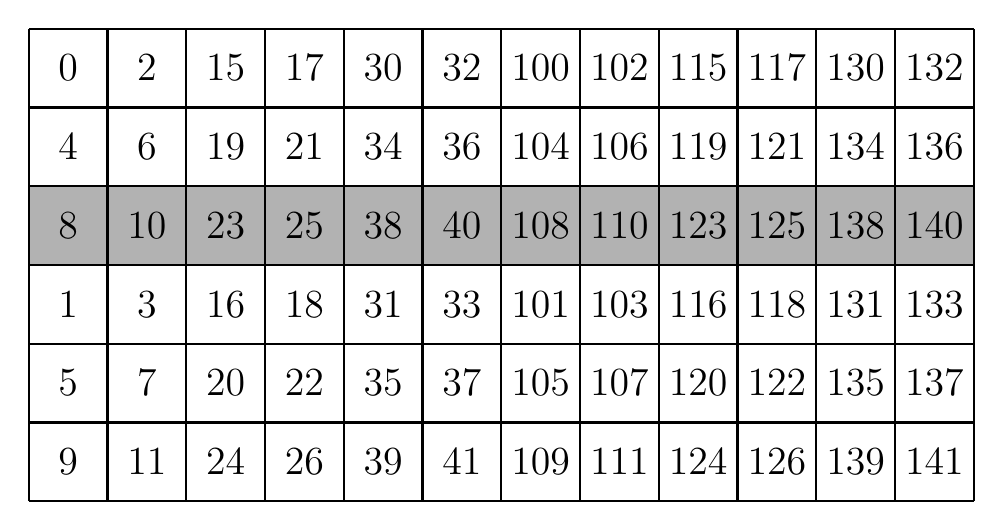
\begin{tikzpicture}[x={(0cm,-1cm)},y={(1cm,0cm)},every node/.style={minimum size=1cm, outer sep=0pt}]
\node[fill=white] at (0,0) {\Large 0};
\node[fill=white] at (0,1) {\Large 2};
\node[fill=white] at (0,2) {\Large 15};
\node[fill=white] at (0,3) {\Large 17};
\node[fill=white] at (0,4) {\Large 30};
\node[fill=white] at (0,5) {\Large 32};
\node[fill=white] at (0,6) {\Large 100};
\node[fill=white] at (0,7) {\Large 102};
\node[fill=white] at (0,8) {\Large 115};
\node[fill=white] at (0,9) {\Large 117};
\node[fill=white] at (0,10) {\Large 130};
\node[fill=white] at (0,11) {\Large 132};
\node[fill=white] at (1,0) {\Large 4};
\node[fill=white] at (1,1) {\Large 6};
\node[fill=white] at (1,2) {\Large 19};
\node[fill=white] at (1,3) {\Large 21};
\node[fill=white] at (1,4) {\Large 34};
\node[fill=white] at (1,5) {\Large 36};
\node[fill=white] at (1,6) {\Large 104};
\node[fill=white] at (1,7) {\Large 106};
\node[fill=white] at (1,8) {\Large 119};
\node[fill=white] at (1,9) {\Large 121};
\node[fill=white] at (1,10) {\Large 134};
\node[fill=white] at (1,11) {\Large 136};
\node[fill=black!30] at (2,0) {\Large 8};
\node[fill=black!30] at (2,1) {\Large 10};
\node[fill=black!30] at (2,2) {\Large 23};
\node[fill=black!30] at (2,3) {\Large 25};
\node[fill=black!30] at (2,4) {\Large 38};
\node[fill=black!30] at (2,5) {\Large 40};
\node[fill=black!30] at (2,6) {\Large 108};
\node[fill=black!30] at (2,7) {\Large 110};
\node[fill=black!30] at (2,8) {\Large 123};
\node[fill=black!30] at (2,9) {\Large 125};
\node[fill=black!30] at (2,10) {\Large 138};
\node[fill=black!30] at (2,11) {\Large 140};
\node[fill=white] at (3,0) {\Large 1};
\node[fill=white] at (3,1) {\Large 3};
\node[fill=white] at (3,2) {\Large 16};
\node[fill=white] at (3,3) {\Large 18};
\node[fill=white] at (3,4) {\Large 31};
\node[fill=white] at (3,5) {\Large 33};
\node[fill=white] at (3,6) {\Large 101};
\node[fill=white] at (3,7) {\Large 103};
\node[fill=white] at (3,8) {\Large 116};
\node[fill=white] at (3,9) {\Large 118};
\node[fill=white] at (3,10) {\Large 131};
\node[fill=white] at (3,11) {\Large 133};
\node[fill=white] at (4,0) {\Large 5};
\node[fill=white] at (4,1) {\Large 7};
\node[fill=white] at (4,2) {\Large 20};
\node[fill=white] at (4,3) {\Large 22};
\node[fill=white] at (4,4) {\Large 35};
\node[fill=white] at (4,5) {\Large 37};
\node[fill=white] at (4,6) {\Large 105};
\node[fill=white] at (4,7) {\Large 107};
\node[fill=white] at (4,8) {\Large 120};
\node[fill=white] at (4,9) {\Large 122};
\node[fill=white] at (4,10) {\Large 135};
\node[fill=white] at (4,11) {\Large 137};
\node[fill=white] at (5,0) {\Large 9};
\node[fill=white] at (5,1) {\Large 11};
\node[fill=white] at (5,2) {\Large 24};
\node[fill=white] at (5,3) {\Large 26};
\node[fill=white] at (5,4) {\Large 39};
\node[fill=white] at (5,5) {\Large 41};
\node[fill=white] at (5,6) {\Large 109};
\node[fill=white] at (5,7) {\Large 111};
\node[fill=white] at (5,8) {\Large 124};
\node[fill=white] at (5,9) {\Large 126};
\node[fill=white] at (5,10) {\Large 139};
\node[fill=white] at (5,11) {\Large 141};
\draw[color=black,thick,shift={(-0.5,-0.5)}] (0,0) grid (6,12);
\end{tikzpicture}
}
\end{adjustbox}
} \\
\hline
$\v{A}(\_,5)$ & $\{32\} \circ (3,2):(4,1)$ &
\scalebox{0.4}{
\begin{adjustbox}{margin=0.5cm}
\scalebox{0.8}{
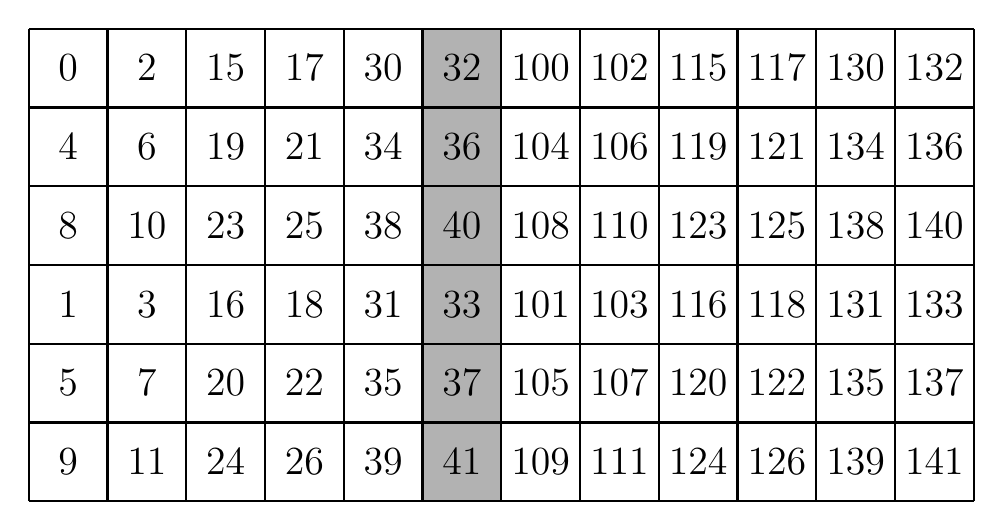
\begin{tikzpicture}[x={(0cm,-1cm)},y={(1cm,0cm)},every node/.style={minimum size=1cm, outer sep=0pt}]
\node[fill=white] at (0,0) {\Large 0};
\node[fill=white] at (0,1) {\Large 2};
\node[fill=white] at (0,2) {\Large 15};
\node[fill=white] at (0,3) {\Large 17};
\node[fill=white] at (0,4) {\Large 30};
\node[fill=black!30] at (0,5) {\Large 32};
\node[fill=white] at (0,6) {\Large 100};
\node[fill=white] at (0,7) {\Large 102};
\node[fill=white] at (0,8) {\Large 115};
\node[fill=white] at (0,9) {\Large 117};
\node[fill=white] at (0,10) {\Large 130};
\node[fill=white] at (0,11) {\Large 132};
\node[fill=white] at (1,0) {\Large 4};
\node[fill=white] at (1,1) {\Large 6};
\node[fill=white] at (1,2) {\Large 19};
\node[fill=white] at (1,3) {\Large 21};
\node[fill=white] at (1,4) {\Large 34};
\node[fill=black!30] at (1,5) {\Large 36};
\node[fill=white] at (1,6) {\Large 104};
\node[fill=white] at (1,7) {\Large 106};
\node[fill=white] at (1,8) {\Large 119};
\node[fill=white] at (1,9) {\Large 121};
\node[fill=white] at (1,10) {\Large 134};
\node[fill=white] at (1,11) {\Large 136};
\node[fill=white] at (2,0) {\Large 8};
\node[fill=white] at (2,1) {\Large 10};
\node[fill=white] at (2,2) {\Large 23};
\node[fill=white] at (2,3) {\Large 25};
\node[fill=white] at (2,4) {\Large 38};
\node[fill=black!30] at (2,5) {\Large 40};
\node[fill=white] at (2,6) {\Large 108};
\node[fill=white] at (2,7) {\Large 110};
\node[fill=white] at (2,8) {\Large 123};
\node[fill=white] at (2,9) {\Large 125};
\node[fill=white] at (2,10) {\Large 138};
\node[fill=white] at (2,11) {\Large 140};
\node[fill=white] at (3,0) {\Large 1};
\node[fill=white] at (3,1) {\Large 3};
\node[fill=white] at (3,2) {\Large 16};
\node[fill=white] at (3,3) {\Large 18};
\node[fill=white] at (3,4) {\Large 31};
\node[fill=black!30] at (3,5) {\Large 33};
\node[fill=white] at (3,6) {\Large 101};
\node[fill=white] at (3,7) {\Large 103};
\node[fill=white] at (3,8) {\Large 116};
\node[fill=white] at (3,9) {\Large 118};
\node[fill=white] at (3,10) {\Large 131};
\node[fill=white] at (3,11) {\Large 133};
\node[fill=white] at (4,0) {\Large 5};
\node[fill=white] at (4,1) {\Large 7};
\node[fill=white] at (4,2) {\Large 20};
\node[fill=white] at (4,3) {\Large 22};
\node[fill=white] at (4,4) {\Large 35};
\node[fill=black!30] at (4,5) {\Large 37};
\node[fill=white] at (4,6) {\Large 105};
\node[fill=white] at (4,7) {\Large 107};
\node[fill=white] at (4,8) {\Large 120};
\node[fill=white] at (4,9) {\Large 122};
\node[fill=white] at (4,10) {\Large 135};
\node[fill=white] at (4,11) {\Large 137};
\node[fill=white] at (5,0) {\Large 9};
\node[fill=white] at (5,1) {\Large 11};
\node[fill=white] at (5,2) {\Large 24};
\node[fill=white] at (5,3) {\Large 26};
\node[fill=white] at (5,4) {\Large 39};
\node[fill=black!30] at (5,5) {\Large 41};
\node[fill=white] at (5,6) {\Large 109};
\node[fill=white] at (5,7) {\Large 111};
\node[fill=white] at (5,8) {\Large 124};
\node[fill=white] at (5,9) {\Large 126};
\node[fill=white] at (5,10) {\Large 139};
\node[fill=white] at (5,11) {\Large 141};
\draw[color=black,thick,shift={(-0.5,-0.5)}] (0,0) grid (6,12);
\end{tikzpicture}
}
\end{adjustbox}
} \\
\hline
$\v{A}(2,((0,\_),\_))$ & $\{8\} \circ (3,2):(15,100)$ &
\scalebox{0.4}{
\begin{adjustbox}{margin=0.5cm}
\scalebox{0.8}{
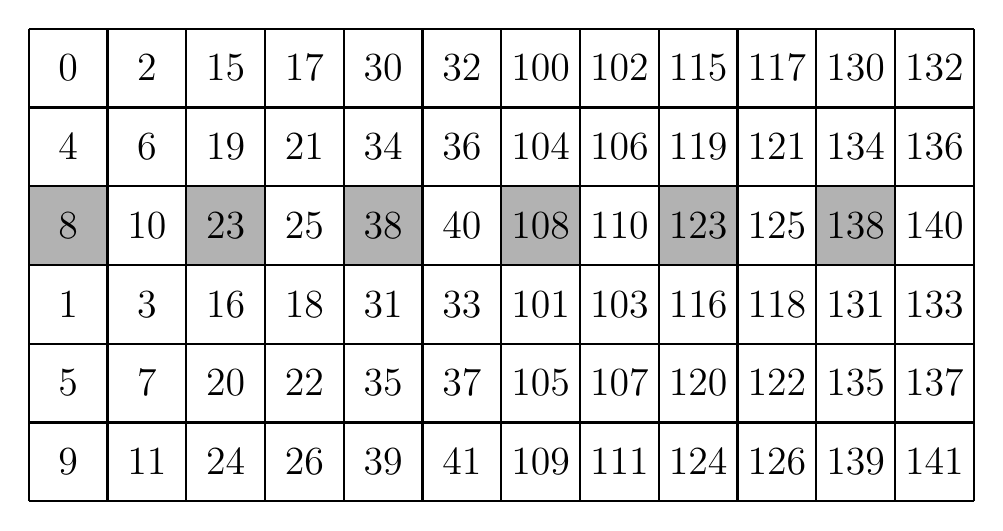
\begin{tikzpicture}[x={(0cm,-1cm)},y={(1cm,0cm)},every node/.style={minimum size=1cm, outer sep=0pt}]
\node[fill=white] at (0,0) {\Large 0};
\node[fill=white] at (0,1) {\Large 2};
\node[fill=white] at (0,2) {\Large 15};
\node[fill=white] at (0,3) {\Large 17};
\node[fill=white] at (0,4) {\Large 30};
\node[fill=white] at (0,5) {\Large 32};
\node[fill=white] at (0,6) {\Large 100};
\node[fill=white] at (0,7) {\Large 102};
\node[fill=white] at (0,8) {\Large 115};
\node[fill=white] at (0,9) {\Large 117};
\node[fill=white] at (0,10) {\Large 130};
\node[fill=white] at (0,11) {\Large 132};
\node[fill=white] at (1,0) {\Large 4};
\node[fill=white] at (1,1) {\Large 6};
\node[fill=white] at (1,2) {\Large 19};
\node[fill=white] at (1,3) {\Large 21};
\node[fill=white] at (1,4) {\Large 34};
\node[fill=white] at (1,5) {\Large 36};
\node[fill=white] at (1,6) {\Large 104};
\node[fill=white] at (1,7) {\Large 106};
\node[fill=white] at (1,8) {\Large 119};
\node[fill=white] at (1,9) {\Large 121};
\node[fill=white] at (1,10) {\Large 134};
\node[fill=white] at (1,11) {\Large 136};
\node[fill=black!30] at (2,0) {\Large 8};
\node[fill=white] at (2,1) {\Large 10};
\node[fill=black!30] at (2,2) {\Large 23};
\node[fill=white] at (2,3) {\Large 25};
\node[fill=black!30] at (2,4) {\Large 38};
\node[fill=white] at (2,5) {\Large 40};
\node[fill=black!30] at (2,6) {\Large 108};
\node[fill=white] at (2,7) {\Large 110};
\node[fill=black!30] at (2,8) {\Large 123};
\node[fill=white] at (2,9) {\Large 125};
\node[fill=black!30] at (2,10) {\Large 138};
\node[fill=white] at (2,11) {\Large 140};
\node[fill=white] at (3,0) {\Large 1};
\node[fill=white] at (3,1) {\Large 3};
\node[fill=white] at (3,2) {\Large 16};
\node[fill=white] at (3,3) {\Large 18};
\node[fill=white] at (3,4) {\Large 31};
\node[fill=white] at (3,5) {\Large 33};
\node[fill=white] at (3,6) {\Large 101};
\node[fill=white] at (3,7) {\Large 103};
\node[fill=white] at (3,8) {\Large 116};
\node[fill=white] at (3,9) {\Large 118};
\node[fill=white] at (3,10) {\Large 131};
\node[fill=white] at (3,11) {\Large 133};
\node[fill=white] at (4,0) {\Large 5};
\node[fill=white] at (4,1) {\Large 7};
\node[fill=white] at (4,2) {\Large 20};
\node[fill=white] at (4,3) {\Large 22};
\node[fill=white] at (4,4) {\Large 35};
\node[fill=white] at (4,5) {\Large 37};
\node[fill=white] at (4,6) {\Large 105};
\node[fill=white] at (4,7) {\Large 107};
\node[fill=white] at (4,8) {\Large 120};
\node[fill=white] at (4,9) {\Large 122};
\node[fill=white] at (4,10) {\Large 135};
\node[fill=white] at (4,11) {\Large 137};
\node[fill=white] at (5,0) {\Large 9};
\node[fill=white] at (5,1) {\Large 11};
\node[fill=white] at (5,2) {\Large 24};
\node[fill=white] at (5,3) {\Large 26};
\node[fill=white] at (5,4) {\Large 39};
\node[fill=white] at (5,5) {\Large 41};
\node[fill=white] at (5,6) {\Large 109};
\node[fill=white] at (5,7) {\Large 111};
\node[fill=white] at (5,8) {\Large 124};
\node[fill=white] at (5,9) {\Large 126};
\node[fill=white] at (5,10) {\Large 139};
\node[fill=white] at (5,11) {\Large 141};
\draw[color=black,thick,shift={(-0.5,-0.5)}] (0,0) grid (6,12);
\end{tikzpicture}
}
\end{adjustbox}
} \\
\hline
$\v{A}((\_,1),(\_,0))$ & $\{1\} \circ (3,(2,3)):(4,(2,15))$ &
\scalebox{0.4}{
\begin{adjustbox}{margin=0.5cm}
\scalebox{0.8}{
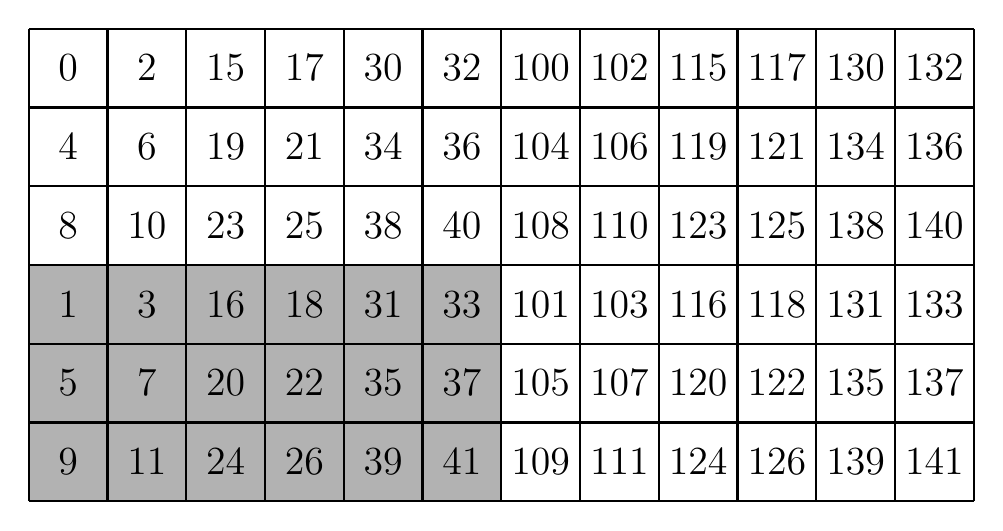
\begin{tikzpicture}[x={(0cm,-1cm)},y={(1cm,0cm)},every node/.style={minimum size=1cm, outer sep=0pt}]
\node[fill=white] at (0,0) {\Large 0};
\node[fill=white] at (0,1) {\Large 2};
\node[fill=white] at (0,2) {\Large 15};
\node[fill=white] at (0,3) {\Large 17};
\node[fill=white] at (0,4) {\Large 30};
\node[fill=white] at (0,5) {\Large 32};
\node[fill=white] at (0,6) {\Large 100};
\node[fill=white] at (0,7) {\Large 102};
\node[fill=white] at (0,8) {\Large 115};
\node[fill=white] at (0,9) {\Large 117};
\node[fill=white] at (0,10) {\Large 130};
\node[fill=white] at (0,11) {\Large 132};
\node[fill=white] at (1,0) {\Large 4};
\node[fill=white] at (1,1) {\Large 6};
\node[fill=white] at (1,2) {\Large 19};
\node[fill=white] at (1,3) {\Large 21};
\node[fill=white] at (1,4) {\Large 34};
\node[fill=white] at (1,5) {\Large 36};
\node[fill=white] at (1,6) {\Large 104};
\node[fill=white] at (1,7) {\Large 106};
\node[fill=white] at (1,8) {\Large 119};
\node[fill=white] at (1,9) {\Large 121};
\node[fill=white] at (1,10) {\Large 134};
\node[fill=white] at (1,11) {\Large 136};
\node[fill=white] at (2,0) {\Large 8};
\node[fill=white] at (2,1) {\Large 10};
\node[fill=white] at (2,2) {\Large 23};
\node[fill=white] at (2,3) {\Large 25};
\node[fill=white] at (2,4) {\Large 38};
\node[fill=white] at (2,5) {\Large 40};
\node[fill=white] at (2,6) {\Large 108};
\node[fill=white] at (2,7) {\Large 110};
\node[fill=white] at (2,8) {\Large 123};
\node[fill=white] at (2,9) {\Large 125};
\node[fill=white] at (2,10) {\Large 138};
\node[fill=white] at (2,11) {\Large 140};
\node[fill=black!30] at (3,0) {\Large 1};
\node[fill=black!30] at (3,1) {\Large 3};
\node[fill=black!30] at (3,2) {\Large 16};
\node[fill=black!30] at (3,3) {\Large 18};
\node[fill=black!30] at (3,4) {\Large 31};
\node[fill=black!30] at (3,5) {\Large 33};
\node[fill=white] at (3,6) {\Large 101};
\node[fill=white] at (3,7) {\Large 103};
\node[fill=white] at (3,8) {\Large 116};
\node[fill=white] at (3,9) {\Large 118};
\node[fill=white] at (3,10) {\Large 131};
\node[fill=white] at (3,11) {\Large 133};
\node[fill=black!30] at (4,0) {\Large 5};
\node[fill=black!30] at (4,1) {\Large 7};
\node[fill=black!30] at (4,2) {\Large 20};
\node[fill=black!30] at (4,3) {\Large 22};
\node[fill=black!30] at (4,4) {\Large 35};
\node[fill=black!30] at (4,5) {\Large 37};
\node[fill=white] at (4,6) {\Large 105};
\node[fill=white] at (4,7) {\Large 107};
\node[fill=white] at (4,8) {\Large 120};
\node[fill=white] at (4,9) {\Large 122};
\node[fill=white] at (4,10) {\Large 135};
\node[fill=white] at (4,11) {\Large 137};
\node[fill=black!30] at (5,0) {\Large 9};
\node[fill=black!30] at (5,1) {\Large 11};
\node[fill=black!30] at (5,2) {\Large 24};
\node[fill=black!30] at (5,3) {\Large 26};
\node[fill=black!30] at (5,4) {\Large 39};
\node[fill=black!30] at (5,5) {\Large 41};
\node[fill=white] at (5,6) {\Large 109};
\node[fill=white] at (5,7) {\Large 111};
\node[fill=white] at (5,8) {\Large 124};
\node[fill=white] at (5,9) {\Large 126};
\node[fill=white] at (5,10) {\Large 139};
\node[fill=white] at (5,11) {\Large 141};
\draw[color=black,thick,shift={(-0.5,-0.5)}] (0,0) grid (6,12);
\end{tikzpicture}
}
\end{adjustbox}
} \\
\hline
$\v{A}((\_,0),((0,\_),1))$ & $\{100\} \circ (3,3):(4,15)$ &
\scalebox{0.4}{
\begin{adjustbox}{margin=0.5cm}
\scalebox{0.8}{
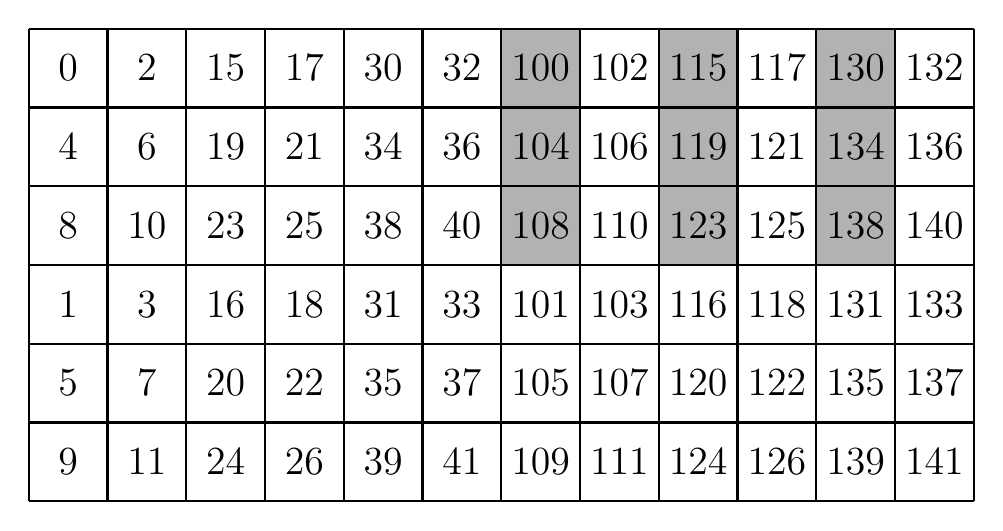
\begin{tikzpicture}[x={(0cm,-1cm)},y={(1cm,0cm)},every node/.style={minimum size=1cm, outer sep=0pt}]
\node[fill=white] at (0,0) {\Large 0};
\node[fill=white] at (0,1) {\Large 2};
\node[fill=white] at (0,2) {\Large 15};
\node[fill=white] at (0,3) {\Large 17};
\node[fill=white] at (0,4) {\Large 30};
\node[fill=white] at (0,5) {\Large 32};
\node[fill=black!30] at (0,6) {\Large 100};
\node[fill=white] at (0,7) {\Large 102};
\node[fill=black!30] at (0,8) {\Large 115};
\node[fill=white] at (0,9) {\Large 117};
\node[fill=black!30] at (0,10) {\Large 130};
\node[fill=white] at (0,11) {\Large 132};
\node[fill=white] at (1,0) {\Large 4};
\node[fill=white] at (1,1) {\Large 6};
\node[fill=white] at (1,2) {\Large 19};
\node[fill=white] at (1,3) {\Large 21};
\node[fill=white] at (1,4) {\Large 34};
\node[fill=white] at (1,5) {\Large 36};
\node[fill=black!30] at (1,6) {\Large 104};
\node[fill=white] at (1,7) {\Large 106};
\node[fill=black!30] at (1,8) {\Large 119};
\node[fill=white] at (1,9) {\Large 121};
\node[fill=black!30] at (1,10) {\Large 134};
\node[fill=white] at (1,11) {\Large 136};
\node[fill=white] at (2,0) {\Large 8};
\node[fill=white] at (2,1) {\Large 10};
\node[fill=white] at (2,2) {\Large 23};
\node[fill=white] at (2,3) {\Large 25};
\node[fill=white] at (2,4) {\Large 38};
\node[fill=white] at (2,5) {\Large 40};
\node[fill=black!30] at (2,6) {\Large 108};
\node[fill=white] at (2,7) {\Large 110};
\node[fill=black!30] at (2,8) {\Large 123};
\node[fill=white] at (2,9) {\Large 125};
\node[fill=black!30] at (2,10) {\Large 138};
\node[fill=white] at (2,11) {\Large 140};
\node[fill=white] at (3,0) {\Large 1};
\node[fill=white] at (3,1) {\Large 3};
\node[fill=white] at (3,2) {\Large 16};
\node[fill=white] at (3,3) {\Large 18};
\node[fill=white] at (3,4) {\Large 31};
\node[fill=white] at (3,5) {\Large 33};
\node[fill=white] at (3,6) {\Large 101};
\node[fill=white] at (3,7) {\Large 103};
\node[fill=white] at (3,8) {\Large 116};
\node[fill=white] at (3,9) {\Large 118};
\node[fill=white] at (3,10) {\Large 131};
\node[fill=white] at (3,11) {\Large 133};
\node[fill=white] at (4,0) {\Large 5};
\node[fill=white] at (4,1) {\Large 7};
\node[fill=white] at (4,2) {\Large 20};
\node[fill=white] at (4,3) {\Large 22};
\node[fill=white] at (4,4) {\Large 35};
\node[fill=white] at (4,5) {\Large 37};
\node[fill=white] at (4,6) {\Large 105};
\node[fill=white] at (4,7) {\Large 107};
\node[fill=white] at (4,8) {\Large 120};
\node[fill=white] at (4,9) {\Large 122};
\node[fill=white] at (4,10) {\Large 135};
\node[fill=white] at (4,11) {\Large 137};
\node[fill=white] at (5,0) {\Large 9};
\node[fill=white] at (5,1) {\Large 11};
\node[fill=white] at (5,2) {\Large 24};
\node[fill=white] at (5,3) {\Large 26};
\node[fill=white] at (5,4) {\Large 39};
\node[fill=white] at (5,5) {\Large 41};
\node[fill=white] at (5,6) {\Large 109};
\node[fill=white] at (5,7) {\Large 111};
\node[fill=white] at (5,8) {\Large 124};
\node[fill=white] at (5,9) {\Large 126};
\node[fill=white] at (5,10) {\Large 139};
\node[fill=white] at (5,11) {\Large 141};
\draw[color=black,thick,shift={(-0.5,-0.5)}] (0,0) grid (6,12);
\end{tikzpicture}
}
\end{adjustbox}
} \\
\hline
$\v{A}((1,\_),((\_,0),\_))$ & $\{4\} \circ (2,(2,2)):(1,(2,100))$ &
\scalebox{0.4}{
\begin{adjustbox}{margin=0.5cm}
\scalebox{0.8}{
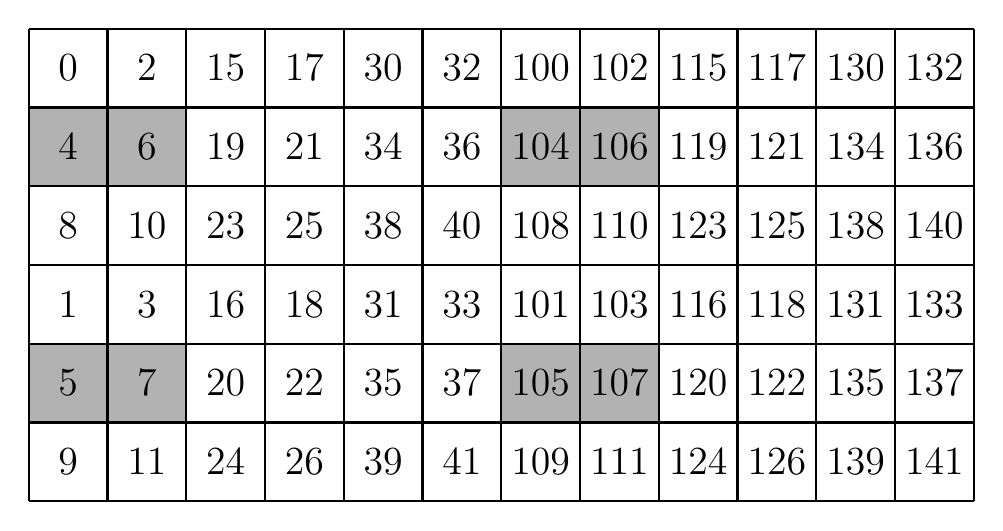
\begin{tikzpicture}[x={(0cm,-1cm)},y={(1cm,0cm)},every node/.style={minimum size=1cm, outer sep=0pt}]
\node[fill=white] at (0,0) {\Large 0};
\node[fill=white] at (0,1) {\Large 2};
\node[fill=white] at (0,2) {\Large 15};
\node[fill=white] at (0,3) {\Large 17};
\node[fill=white] at (0,4) {\Large 30};
\node[fill=white] at (0,5) {\Large 32};
\node[fill=white] at (0,6) {\Large 100};
\node[fill=white] at (0,7) {\Large 102};
\node[fill=white] at (0,8) {\Large 115};
\node[fill=white] at (0,9) {\Large 117};
\node[fill=white] at (0,10) {\Large 130};
\node[fill=white] at (0,11) {\Large 132};
\node[fill=black!30] at (1,0) {\Large 4};
\node[fill=black!30] at (1,1) {\Large 6};
\node[fill=white] at (1,2) {\Large 19};
\node[fill=white] at (1,3) {\Large 21};
\node[fill=white] at (1,4) {\Large 34};
\node[fill=white] at (1,5) {\Large 36};
\node[fill=black!30] at (1,6) {\Large 104};
\node[fill=black!30] at (1,7) {\Large 106};
\node[fill=white] at (1,8) {\Large 119};
\node[fill=white] at (1,9) {\Large 121};
\node[fill=white] at (1,10) {\Large 134};
\node[fill=white] at (1,11) {\Large 136};
\node[fill=white] at (2,0) {\Large 8};
\node[fill=white] at (2,1) {\Large 10};
\node[fill=white] at (2,2) {\Large 23};
\node[fill=white] at (2,3) {\Large 25};
\node[fill=white] at (2,4) {\Large 38};
\node[fill=white] at (2,5) {\Large 40};
\node[fill=white] at (2,6) {\Large 108};
\node[fill=white] at (2,7) {\Large 110};
\node[fill=white] at (2,8) {\Large 123};
\node[fill=white] at (2,9) {\Large 125};
\node[fill=white] at (2,10) {\Large 138};
\node[fill=white] at (2,11) {\Large 140};
\node[fill=white] at (3,0) {\Large 1};
\node[fill=white] at (3,1) {\Large 3};
\node[fill=white] at (3,2) {\Large 16};
\node[fill=white] at (3,3) {\Large 18};
\node[fill=white] at (3,4) {\Large 31};
\node[fill=white] at (3,5) {\Large 33};
\node[fill=white] at (3,6) {\Large 101};
\node[fill=white] at (3,7) {\Large 103};
\node[fill=white] at (3,8) {\Large 116};
\node[fill=white] at (3,9) {\Large 118};
\node[fill=white] at (3,10) {\Large 131};
\node[fill=white] at (3,11) {\Large 133};
\node[fill=black!30] at (4,0) {\Large 5};
\node[fill=black!30] at (4,1) {\Large 7};
\node[fill=white] at (4,2) {\Large 20};
\node[fill=white] at (4,3) {\Large 22};
\node[fill=white] at (4,4) {\Large 35};
\node[fill=white] at (4,5) {\Large 37};
\node[fill=black!30] at (4,6) {\Large 105};
\node[fill=black!30] at (4,7) {\Large 107};
\node[fill=white] at (4,8) {\Large 120};
\node[fill=white] at (4,9) {\Large 122};
\node[fill=white] at (4,10) {\Large 135};
\node[fill=white] at (4,11) {\Large 137};
\node[fill=white] at (5,0) {\Large 9};
\node[fill=white] at (5,1) {\Large 11};
\node[fill=white] at (5,2) {\Large 24};
\node[fill=white] at (5,3) {\Large 26};
\node[fill=white] at (5,4) {\Large 39};
\node[fill=white] at (5,5) {\Large 41};
\node[fill=white] at (5,6) {\Large 109};
\node[fill=white] at (5,7) {\Large 111};
\node[fill=white] at (5,8) {\Large 124};
\node[fill=white] at (5,9) {\Large 126};
\node[fill=white] at (5,10) {\Large 139};
\node[fill=white] at (5,11) {\Large 141};
\draw[color=black,thick,shift={(-0.5,-0.5)}] (0,0) grid (6,12);
\end{tikzpicture}
}
\end{adjustbox}
} \\
\hline
\end{tabular}
\caption{沿逻辑子边界切片以提取子张量的 $6 {\times} 12$ 张量。}
\label{fig:slicing}
\end{figure}

图~\ref{fig:slicing} 展示了在一个 $6 {\times} 12$ 矩阵中切片以提取行、列与子矩阵的示例。这些示例使用记号 $\{a\}$ 表示的计数迭代器访问器，以指明偏移 $a \in \Z$。切片的过程包括向张量偏移做累加，并确定布局中尚未求值的部分。

在许多张量库（如 {\tt numpy.ndarray}、{\tt torch.tensor} 和 MATLAB）中，切片以与上面类似的记法得到支持：写 {\tt my\_matrix[2,:]} 提取矩阵的第二行，写 {\tt my\_matrix[:,4]} 提取矩阵的第四列。这些库还支持范围切片（ranged slicing），例如 {\tt my\_matrix[2:4,1:3]} 提取从第二行到第四行、从第一列到第三列的子矩阵。\CuTe 不支持范围切片，因为它认为范围切片存在若干问题：
\begin{compactitem}
\item 范围切片无法表达图~\ref{fig:slicing} 中演示的所有切片。最后一个切片示例就无法仅凭矩阵行与列上的范围切片来表达。
\item 范围切片助长如下模式
\begin{python}
# 为每个 thr_id 提取 TILE_SIZE 大小的数据
thr_data = my_data[thr_id*TILE_SIZE:(thr_id+1)*TILE_SIZE]
\end{python}
来获取每个线程局部的一块数据“瓦片”（tile）。这种模式把 {\tt TILE\_SIZE}（通常正是程序想要在其上做优化的静态常量）与 {\tt thr\_id}（本质上是每个线程局部的动态索引）混为一谈。与之相反，\CuTe 更倾向于两阶段的“重排—切片”方法，例如
\begin{python}
# 将 my_data 张量重排并重塑为形状 (TILE_SIZE,NumTiles)
# 这是对更一般的 composition(my_data, Transform_Layout) 的封装
tiled_data = logical_divide(my_data, TILE_SIZE)  # (TILE_SIZE, NumTiles)
assert size[1](tiled_data) == NumThrs            # 验证 NumTiles == NumThrs
# 对铺瓦后的张量切片，取 thr_id 局部的 TILE_SIZE 数据
thr_data = thr_tile_data[None, thr_id]           # TILE_SIZE
\end{python}
它把 {\tt TILE\_SIZE} 与 {\tt thr\_id} 这两个性质不同的参数分开，更容易让编译器据此推理并传播静态信息（例如 {\tt thr\_data} 的大小为 {\tt TILE\_SIZE}），而且同样灵活。关于通用分块（partitioning）的细节与示例见第~\ref{sec:layouttv} 节，关于逻辑切分（logical divide）的细节与示例见第~\ref{sec:logical_divide} 节。
\item 范围切片能够表达一些无法用 \CuTe 布局表示的切片。例如，取图~\ref{fig:slicing} 中的 $\v{A}$，切片 {\tt $\v{A}$(0,0:2:12)} 可以得到 $\{0\} \circ (3,2):(15,100)$，而切片 {\tt $\v{A}$(0:2:6,0)} 由于所请求的切片与 $\v{A}$ 的布局不相容而无法表示。这主要是由于所请求的瓦片与张量布局不相容，因此我们更希望这一错误在“重排—重塑”阶段（{\tt composition}）就被检测并暴露出来，而不是留到切片阶段。关于布局群复合可采纳性条件的细节与示例，见第~\ref{sec:composition_impl} 节。
\end{compactitem}
